\documentclass[11pt, xcolor=dvipsnames]{beamer}

% --- Codificação e idioma (XeLaTeX) ---
\usepackage{fontspec}
\usepackage{polyglossia}
\setdefaultlanguage{brazil}

% --- Matemática ---
\usepackage{amsmath, amssymb, amsfonts}
\usepackage{mathtools}

% --- Links ---
\usepackage{hyperref}

% --- Gráficos / figuras / tabelas ---
\usepackage{graphicx}
\graphicspath{{../new-plantuml/}}
\usepackage{booktabs}
\usepackage{array}
\usepackage{adjustbox}
\usepackage{multirow}

% --- Cores e caixas (ênfase) ---
\usepackage{xcolor}
\usepackage[most]{tcolorbox}

% --- Layout e tipografia ---
\usepackage[document]{ragged2e}

% --- TikZ/pgf ---
\usepackage{tikz}
\usetikzlibrary{arrows,positioning,fit,calc,shapes.geometric}
\usepackage{pgfplots}
\pgfplotsset{compat=1.15}

\usefonttheme[onlymath]{serif}

% === PALETA CLARA (tema acadêmico) ===
\definecolor{fundo}{RGB}{250,250,250}
% Paleta verde original (comentada para teste):
% \definecolor{verde}{RGB}{0,100,70}
% \definecolor{verdeClaro}{RGB}{46,140,100}
% Paleta azul (experimental):
\definecolor{verde}{RGB}{0,82,147}        % Azul profundo (era verde escuro)
\definecolor{verdeClaro}{RGB}{65,131,196} % Azul médio (era verde claro)
\definecolor{textoBase}{RGB}{35,35,35}
\definecolor{amarelo}{RGB}{200,150,0}
\definecolor{laranja}{RGB}{210,100,0}
\definecolor{azulEscuro}{RGB}{30,60,90}

\usetheme{Darmstadt}
\useoutertheme{miniframes}
\useinnertheme[shadow=true]{rounded}
\setbeamertemplate{navigation symbols}{}

% Plano de fundo e texto
\setbeamercolor{background canvas}{bg=fundo}
\setbeamercolor{normal text}{fg=textoBase,bg=fundo}

% Estrutura e títulos
\setbeamercolor{structure}{fg=verdeClaro}
\setbeamercolor{title}{bg=verde,fg=white}
\setbeamercolor{frametitle}{fg=verde, bg=verde!15!fundo}

% Blocos
\setbeamercolor{block title}{bg=verde,fg=white}
\setbeamercolor{block body}{bg=fundo!90!verde,fg=textoBase}

% Bullets
\setbeamercolor{itemize item}{fg=verde}
\setbeamercolor{itemize subitem}{fg=verdeClaro}
\setbeamercolor{enumerate item}{fg=verde}

% Rodapé (escurecido)
\setbeamercolor{author in head/foot}{bg=verde!40!fundo,fg=textoBase!40!black}
\setbeamercolor{title in head/foot}{bg=verde!40!fundo,fg=textoBase!40!black}
\setbeamercolor{date in head/foot}{bg=verde!40!fundo,fg=textoBase!40!black}

% Mini-frames (indicadores de seção - escurecido)
\setbeamercolor{mini frame}{fg=verde,bg=verde!50}
\setbeamercolor{section in head/foot}{fg=textoBase,bg=verde!35!fundo}

% Utilitários
\newcommand{\intsize}{\fontsize{8}{11}\selectfont}
\newcommand{\evensmaller}{\fontsize{6.6}{11}\selectfont}
\newcommand{\destaque}[1]{\textbf{\textcolor{verde}{#1}}}
\newcommand{\sutil}[1]{\textcolor{textoBase!60}{#1}}

% Rodapé com contagem de slides
\makeatletter
\defbeamertemplate*{footline}{infolines theme}{%
  \leavevmode%
  \hbox{%
    \begin{beamercolorbox}[wd=.33\paperwidth,ht=2.25ex,dp=1ex,center]{author in head/foot}%
      \usebeamerfont{author in head/foot}\insertshortauthor
    \end{beamercolorbox}%
    \begin{beamercolorbox}[wd=.34\paperwidth,ht=2.25ex,dp=1ex,center]{title in head/foot}%
      \usebeamerfont{title in head/foot}\insertshorttitle
    \end{beamercolorbox}%
    \begin{beamercolorbox}[wd=.33\paperwidth,ht=2.25ex,dp=1ex,right]{date in head/foot}%
      \usebeamerfont{date in head/foot}\insertshortdate{}\hspace*{2em}%
      \sutil{\insertframenumber{}} \hspace*{2ex}
    \end{beamercolorbox}%
  }%
  \vskip0pt%
}
\makeatother
\setbeamertemplate{footline}[infolines theme]

\newtcolorbox{calloutbox}{
  colback=verde!5!fundo,
  colframe=verde!70,
  boxrule=0.6pt, arc=2pt, left=4pt,right=4pt,top=3pt,bottom=3pt
}

\newtcolorbox{alertbox}{
  colback=laranja!8!fundo,
  colframe=laranja!80,
  boxrule=0.6pt, arc=2pt, left=4pt,right=4pt,top=3pt,bottom=3pt
}

% --- Metadados ---
\title[\sutil{DQN-ILS}]{DQN-ILS: Deep Q-Network para \\ Iterated Local Search no TSP}
\author[\sutil{Grupo RL-CO}]{\intsize \textbf{Leonardo Assumpção}, \textbf{Gabriel Souto} \\ \sutil{Lucas Barbosa, Matheus Bastos, Rafael Dias}}
\institute[UFRJ]{\intsize PESC/COPPE/UFRJ -- OTIMIA (COS887)}
\date[]{\sutil{Dezembro/2025}}

% Sumário por seção
\AtBeginSection[]{
  \begin{frame}[noframenumbering]
    \frametitle{Sumário}
    \tableofcontents[currentsection, hideallsubsections]
  \end{frame}
}

\begin{document}

% ----------------- CAPA -----------------
\maketitle

% ======================================================
\section{Introdução}
% ======================================================

\begin{frame}{Motivação}
  \footnotesize
  \begin{itemize}
    \item O \destaque{TSP} (Traveling Salesman Problem) é NP-difícil com vasta aplicação prática.
    \item \destaque{Iterated Local Search (ILS)} combina perturbações e buscas locais.
    \item Múltiplas estratégias disponíveis: qual usar em cada momento?
  \end{itemize}
  \vspace{3mm}
  \begin{calloutbox}
    {\footnotesize
    \textbf{Pergunta central}: Podemos usar \destaque{Deep Reinforcement Learning} para aprender \emph{qual combinação} de estratégias funciona melhor em cada situação?
    }
  \end{calloutbox}
  \vspace{2mm}
  \begin{alertbox}
    {\scriptsize
    \textbf{Evolução}: Q-Learning tabular $\rightarrow$ \destaque{Deep Q-Network (DQN)} \\
    Estado contínuo, aproximação por rede neural, experience replay.
    }
  \end{alertbox}
\end{frame}

\begin{frame}{Objetivos}
  \footnotesize
  \begin{enumerate}
    \item Propor uma abordagem híbrida \destaque{DQN-ILS} que integra Deep Q-Network ao framework do Iterated Local Search.
    \item \destaque{Aprender} a partir de episódios de treino qual combinação (perturbação + busca local) tende a melhorar soluções.
    \item \destaque{Avaliar} se a política aprendida generaliza para instâncias não vistas.
    \item \destaque{Comparar} Standard DQN vs Double DQN.
  \end{enumerate}
  \vspace{4mm}
  \begin{calloutbox}
    {\scriptsize
    Foco em reduzir o \emph{gap} relativo ao baseline de forma automática.
    }
  \end{calloutbox}
\end{frame}

% ======================================================
\section{Fundamentos}
% ======================================================

\begin{frame}{O Problema: TSP}
  \footnotesize
  \textbf{Traveling Salesman Problem:}
  \vspace{2mm}
  \begin{itemize}
    \item Dado um conjunto de $n$ cidades e distâncias $d_{ij}$, encontrar o \destaque{tour de menor custo}.
  \end{itemize}
  \vspace{2mm}
  \[
    \min_{\pi} \sum_{i=1}^{n} d_{\pi(i), \pi(i+1)} \quad \big( \pi(n+1) = \pi(1) \big)
  \]
  \vspace{2mm}
  \begin{columns}[T]
    \begin{column}{0.47\textwidth}
      \begin{itemize}
        \item Complexidade: \destaque{NP-difícil}
        \item Soluções exatas: impraticáveis para $n$ grande
        \item Alternativa: heurísticas e meta-heurísticas
      \end{itemize}
    \end{column}
    \begin{column}{0.53\textwidth}
      \centering
      \begin{tikzpicture}[scale=0.65]
        \foreach \i/\x/\y in {1/0/0, 2/1.5/2, 3/3/0.5, 4/2.5/3, 5/4/2} {
          \node[circle, fill=verde, inner sep=2pt, text=white, font=\tiny] (\i) at (\x,\y) {\i};
        }
        \draw[thick, verde!70] (1) -- (2) -- (4) -- (5) -- (3) -- (1);
      \end{tikzpicture}
      \vspace{1mm}
      {\scriptsize \sutil{Exemplo: tour com 5 cidades}}
    \end{column}
  \end{columns}
\end{frame}

\begin{frame}{Iterated Local Search (ILS)}
  \footnotesize
  \begin{columns}[T]
    \begin{column}{0.47\textwidth}
      \textbf{Estrutura básica:}
      \begin{enumerate}
        \item Gerar solução inicial $s_0$
        \item Aplicar busca local: $s \leftarrow \text{BL}(s_0)$
        \item Repetir até limite de tempo:
          \begin{itemize}
            \item Perturbar: $s' \leftarrow \text{Pert}(s)$
            \item Refinar: $s'' \leftarrow \text{BL}(s')$
            \item Aceitar se melhora
          \end{itemize}
        \item Retornar melhor solução
      \end{enumerate}
    \end{column}
    \begin{column}{0.53\textwidth}
      \begin{calloutbox}
        {\scriptsize
        \textbf{Componentes intercambiáveis:} \\[1mm]
        Múltiplas perturbações e buscas locais podem ser combinadas. \\[2mm]
        \destaque{DQN aprende a escolher dinamicamente!}
        }
      \end{calloutbox}
    \end{column}
  \end{columns}
\end{frame}

\begin{frame}{Deep Q-Network (DQN)}
  \footnotesize
  \begin{columns}[T]
    \begin{column}{0.55\textwidth}
      \textbf{Principais características:}
      \begin{itemize}
        \item Aproxima $Q(s,a)$ com rede neural
        \item \destaque{Experience Replay}: armazena transições $(s, a, r, s')$ em buffer
        \item \destaque{Target Network}: rede separada para estabilidade
        \item Treino off-policy com mini-batches
      \end{itemize}
      \vspace{2mm}
      \textbf{Update:}
      \[
        L = \mathbb{E}\left[(y - Q_\theta(s,a))^2\right]
      \]
    \end{column}
    \begin{column}{0.45\textwidth}
      \begin{alertbox}
        {\scriptsize
        \textbf{Standard DQN:} \\
        $y = r + \gamma \max_{a'} Q_{\theta^-}(s', a')$ \\[3mm]
        \textbf{Double DQN:} \\
        $a^* = \arg\max_{a'} Q_\theta(s', a')$ \\
        $y = r + \gamma Q_{\theta^-}(s', a^*)$ \\[2mm]
        \sutil{Reduz superestimação de Q-values}
        }
      \end{alertbox}
    \end{column}
  \end{columns}
\end{frame}

% ======================================================
\section{Modelagem MDP}
% ======================================================

\begin{frame}{Modelagem como MDP}
  \footnotesize
  \vspace{-2mm}
  \begin{calloutbox}
    {\footnotesize
    \textbf{MDP}: Processo de Decisão de Markov $(S, A, T, R)$
    }
  \end{calloutbox}
  \vspace{2mm}
  \begin{itemize}
    \setlength{\itemsep}{2pt}
    \item \destaque{Estado $s$}: vetor contínuo de 19 dimensões
    \item \destaque{Ação $a$}: combinação (perturbação, busca local)
    \item \destaque{Transição $T$}: aprendida implicitamente via experience replay
    \item \destaque{Recompensa $R$}: baseada em melhoria do gap
  \end{itemize}
  \vspace{2mm}
  \centering
  % Diagrama: dqn_mdp_mapping.png
  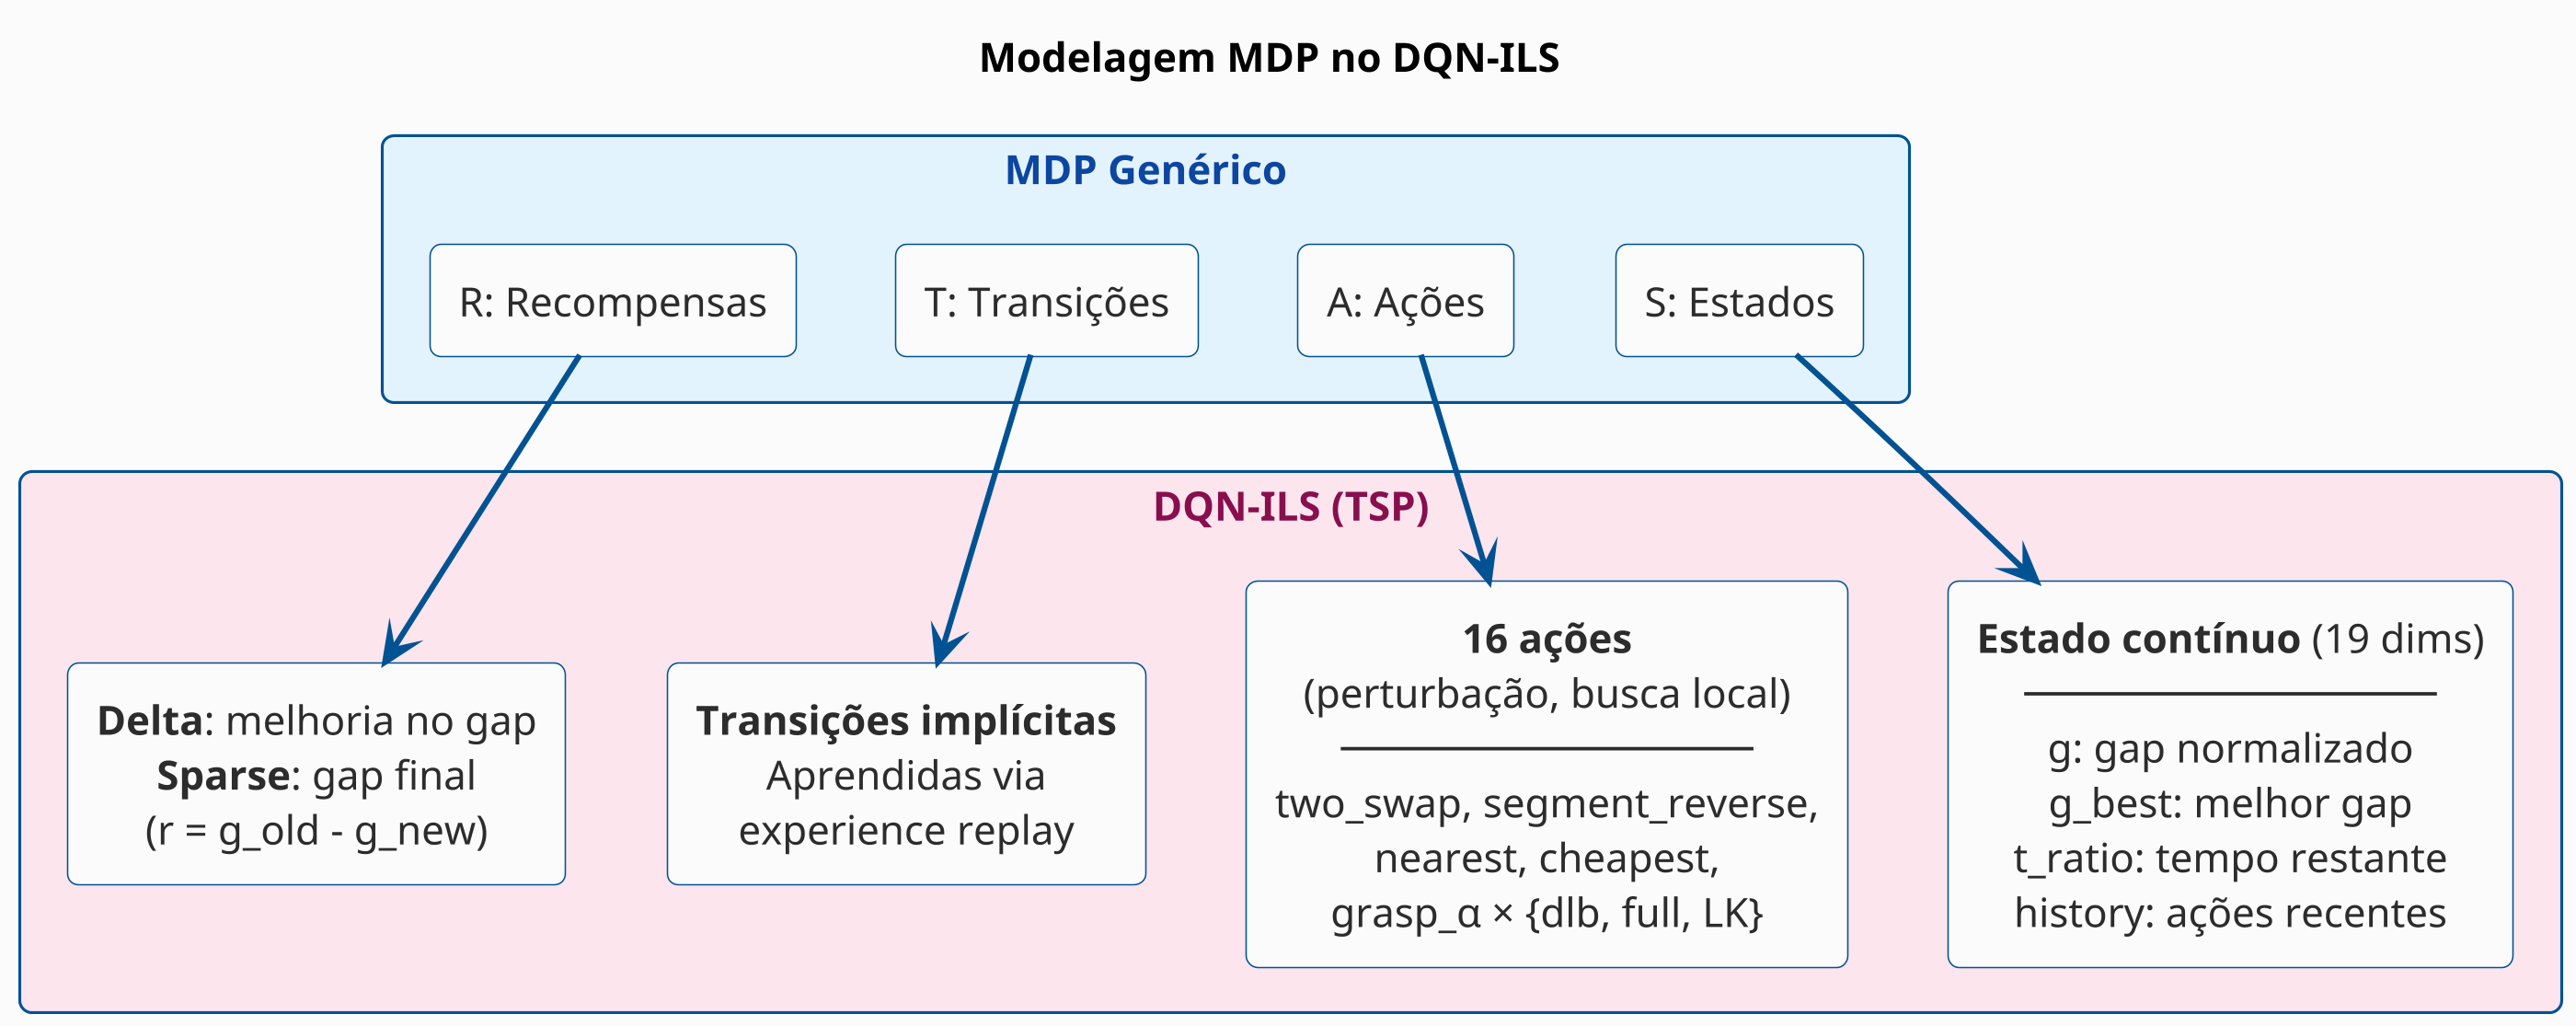
\includegraphics[width=0.85\textwidth,height=0.38\textheight,keepaspectratio]{dqn_mdp_mapping.png}
\end{frame}

\begin{frame}{Representação de Estado}
  \footnotesize
  \textbf{Estado contínuo} (19 dimensões):
  \vspace{2mm}

  \centering
  \renewcommand{\arraystretch}{1.3}
  \begin{tabular}{clc}
    \toprule
    \textbf{Componente} & \textbf{Descrição} & \textbf{Dimensão} \\
    \midrule
    $g$ & Gap atual normalizado & 1 \\
    $g_{\text{best}}$ & Melhor gap do episódio & 1 \\
    $t_{\text{ratio}}$ & Tempo restante / $T$ & 1 \\
    history & Últimas ações (one-hot) & 16 \\
    \midrule
    \multicolumn{2}{r}{\textbf{Total}} & \textbf{19} \\
    \bottomrule
  \end{tabular}
  \vspace{3mm}

  \begin{calloutbox}
    {\scriptsize
    \textbf{Normalização do gap:} $\text{norm}(g) = \text{sign}(g) \cdot \frac{\log(1 + |g|)}{\log(101)}$ \\[1mm]
    Transforma escala logarítmica, simétrico para gaps negativos.
    }
  \end{calloutbox}
\end{frame}

\begin{frame}{Espaço de Ações}
  \footnotesize
  \textbf{16 ações} = combinações de perturbação + busca local:
  \vspace{2mm}

  \centering
  \renewcommand{\arraystretch}{1.1}
  \begin{tabular}{clll}
    \toprule
    \textbf{Ação} & \textbf{Perturbação} & \textbf{Busca Local} & \textbf{Característica} \\
    \midrule
    0-2 & two\_swap & dlb, full, LK & Perturbação leve \\
    3-4 & segment\_reverse & dlb, full & Perturbação leve \\
    5-7 & nearest & dlb, full, LK & Restart com NN \\
    8-9 & cheapest & dlb, full & Restart com CI \\
    10-11 & grasp\_0.03 & dlb, full & GRASP quase-guloso \\
    12-13 & grasp\_0.1 & dlb, full & GRASP balanceado \\
    14-15 & grasp\_0.3 & dlb, full & GRASP diversificado \\
    \bottomrule
  \end{tabular}
  \vspace{3mm}

  \begin{alertbox}
    {\scriptsize
    \textbf{Variantes de 2-opt:} \\
    \textbf{dlb}: Don't Look Bits (rápido) | \textbf{full}: $O(n^2)$ (melhor) | \textbf{LK}: Lin-Kernighan
    }
  \end{alertbox}
\end{frame}

\begin{frame}{Função de Recompensa}
  \footnotesize
  \begin{columns}[T]
    \begin{column}{0.5\textwidth}
      \textbf{Delta Reward} (padrão):
      \[
        r = g_{\text{best}}^{\text{old}} - g_{\text{best}}^{\text{new}}
      \]
      \begin{itemize}
        \item Positiva apenas quando melhora o recorde
        \item Recompensa incremental por step
        \item Sinal mais frequente durante treino
      \end{itemize}
    \end{column}
    \begin{column}{0.5\textwidth}
      \textbf{Sparse Reward}:
      \[
        r = \begin{cases}
          0 & \text{durante episódio} \\
          -\text{norm}(g_{\text{best}}) & \text{no final}
        \end{cases}
      \]
      \begin{itemize}
        \item Recompensa apenas no fim
        \item Menor gap $\rightarrow$ maior reward
        \item Credit assignment mais difícil
      \end{itemize}
    \end{column}
  \end{columns}
  \vspace{3mm}
  \begin{calloutbox}
    {\scriptsize
    \textbf{Baseline}: Gap calculado relativo a GRASP+2opt (não ao ótimo). \\
    Garante distribuição consistente entre treino e teste.
    }
  \end{calloutbox}
\end{frame}

% ======================================================
\section{Arquitetura}
% ======================================================

\begin{frame}{Arquitetura da Q-Network}
  \footnotesize
  \centering
  % Diagrama: dqn_architecture.png
  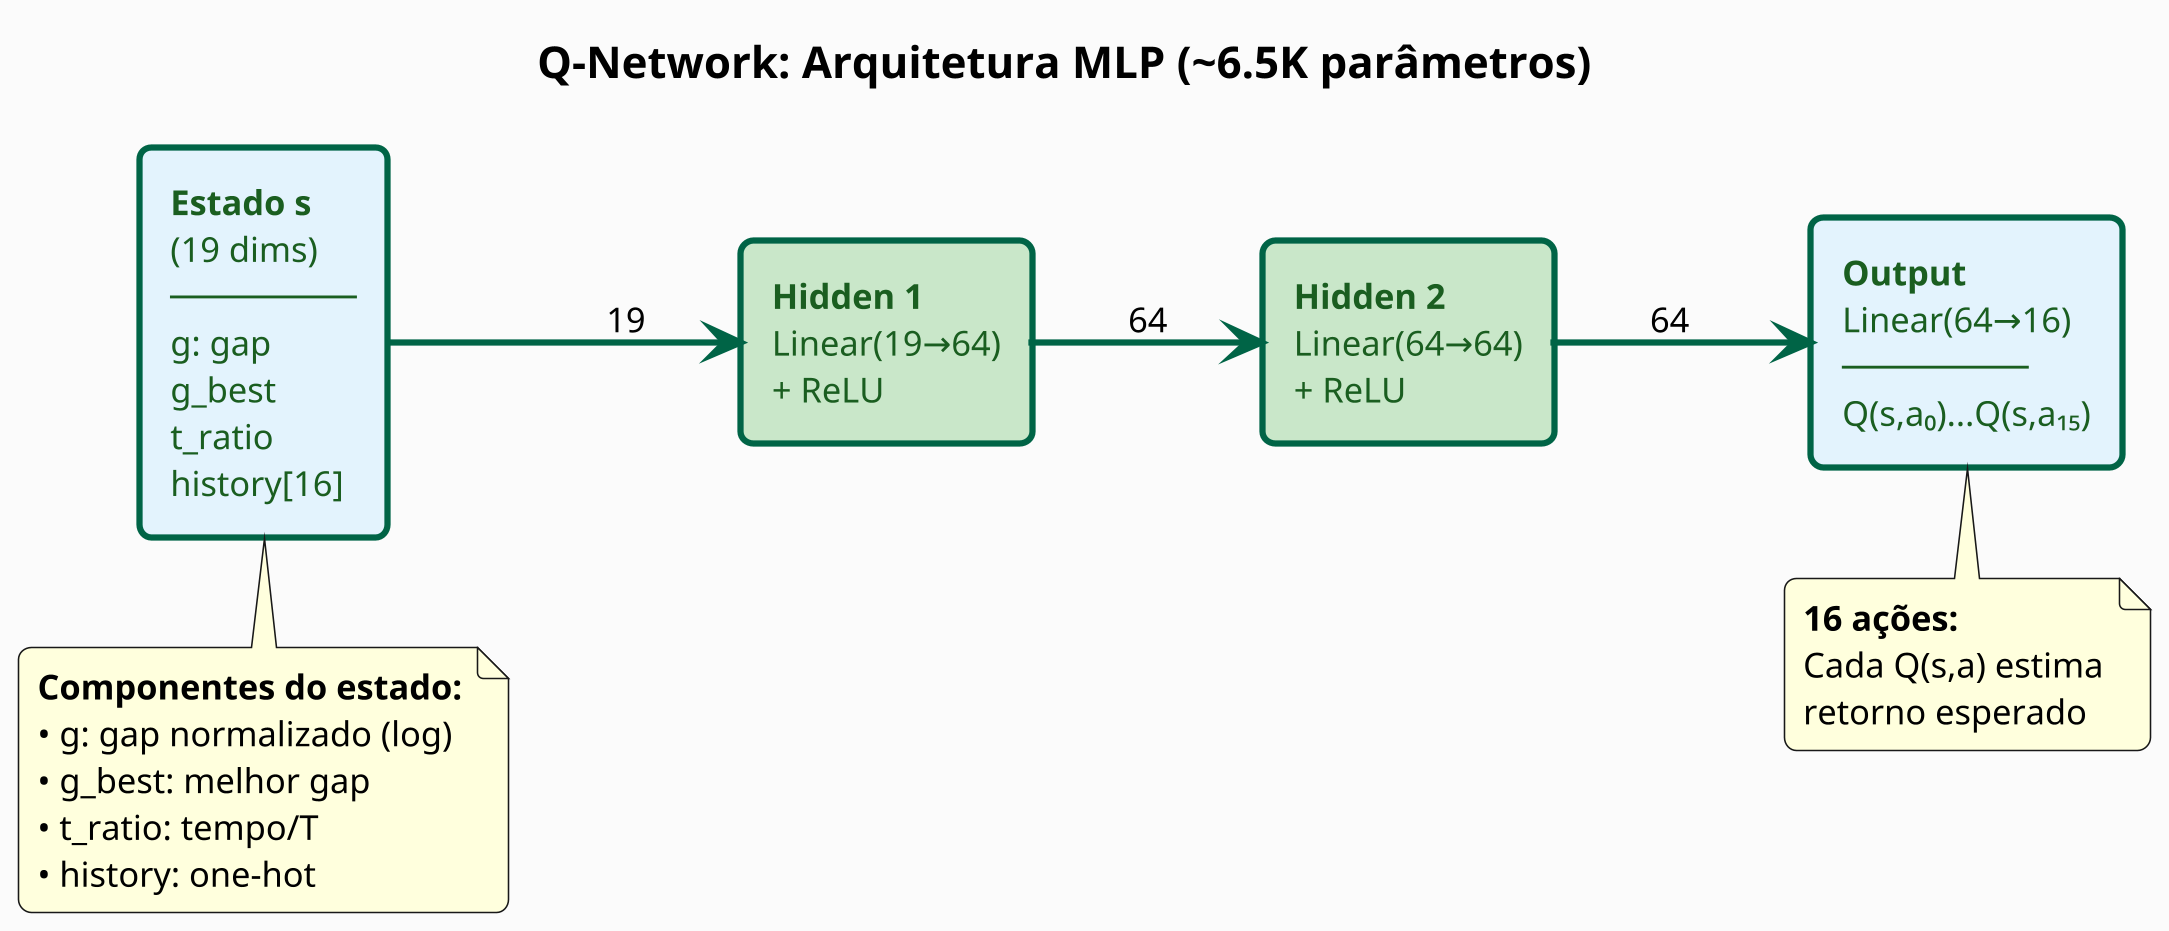
\includegraphics[width=0.9\textwidth,height=0.55\textheight,keepaspectratio]{dqn_architecture.png}
  \vspace{3mm}

  \begin{columns}[T]
    \begin{column}{0.5\textwidth}
      \begin{calloutbox}
        {\scriptsize
        \textbf{Arquitetura MLP:} \\
        Input (19) $\rightarrow$ Linear(64) $\rightarrow$ ReLU \\
        $\rightarrow$ Linear(64) $\rightarrow$ ReLU $\rightarrow$ Linear(16)
        }
      \end{calloutbox}
    \end{column}
    \begin{column}{0.5\textwidth}
      \begin{alertbox}
        {\scriptsize
        \textbf{Características:} \\
        $\sim$6.5K parâmetros total \\
        Leve e eficiente para inferência
        }
      \end{alertbox}
    \end{column}
  \end{columns}
\end{frame}

\begin{frame}{Standard DQN vs Double DQN}
  \footnotesize
  \begin{columns}[T]
    \begin{column}{0.5\textwidth}
      \centering
      \begin{tcolorbox}[
        colback=verde!5!fundo,
        colframe=verde!60!verdeClaro,
        arc=4pt,
        boxrule=1pt,
        width=0.95\textwidth,
        halign=center
      ]
        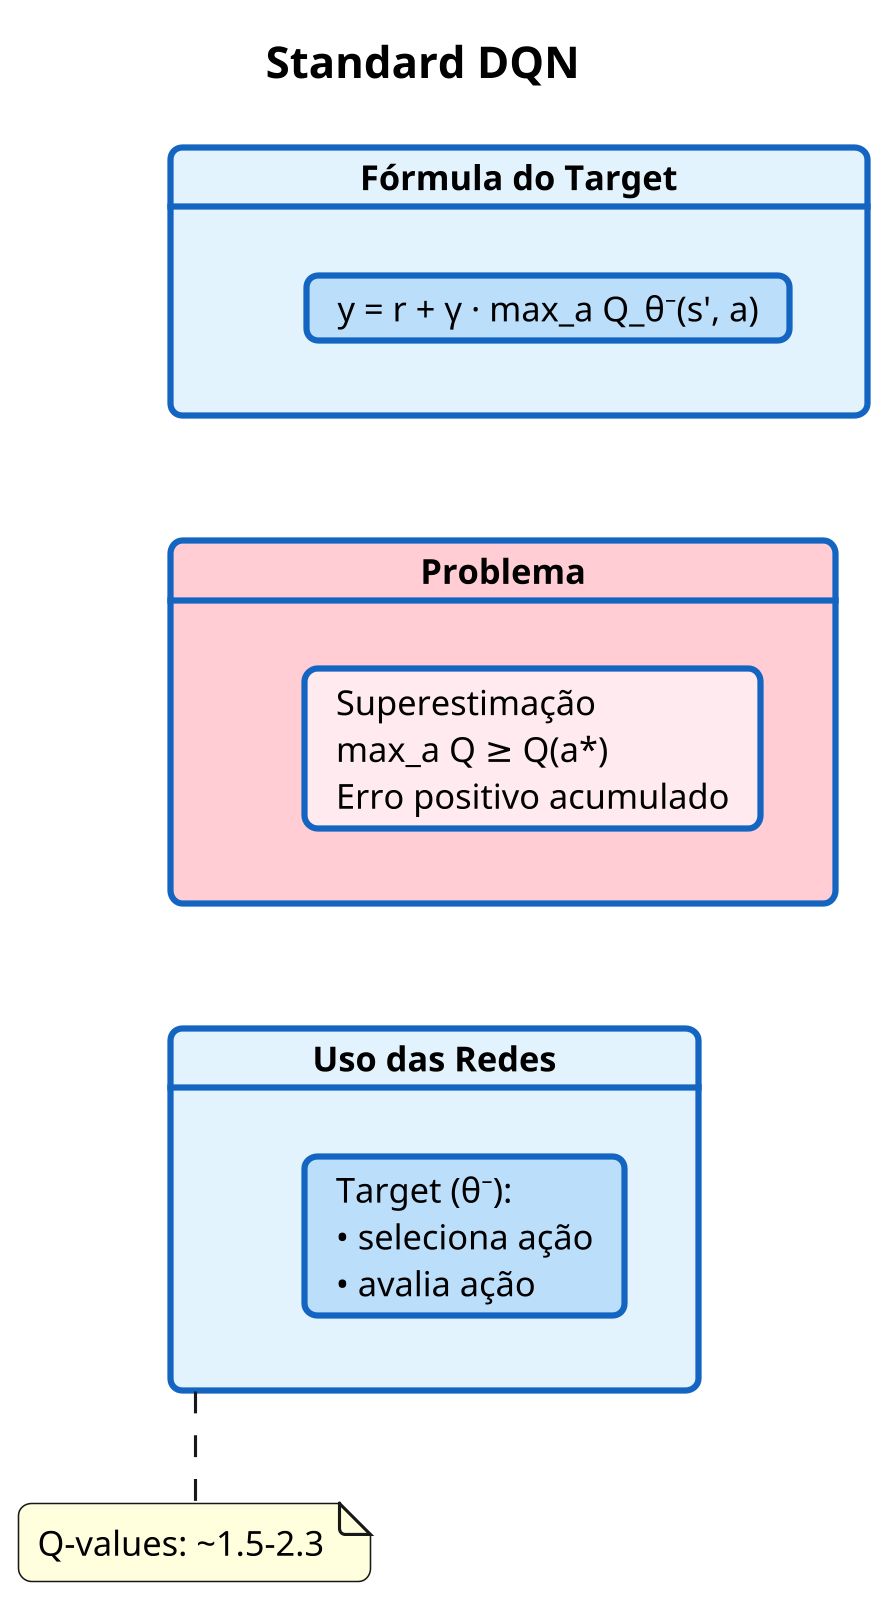
\includegraphics[width=0.95\textwidth,height=0.58\textheight,keepaspectratio]{standard_dqn.png}
      \end{tcolorbox}
    \end{column}
    \begin{column}{0.5\textwidth}
      \centering
      \begin{tcolorbox}[
        colback=verde!5!fundo,
        colframe=verde!60!verdeClaro,
        arc=4pt,
        boxrule=1pt,
        width=0.95\textwidth,
        halign=center
      ]
        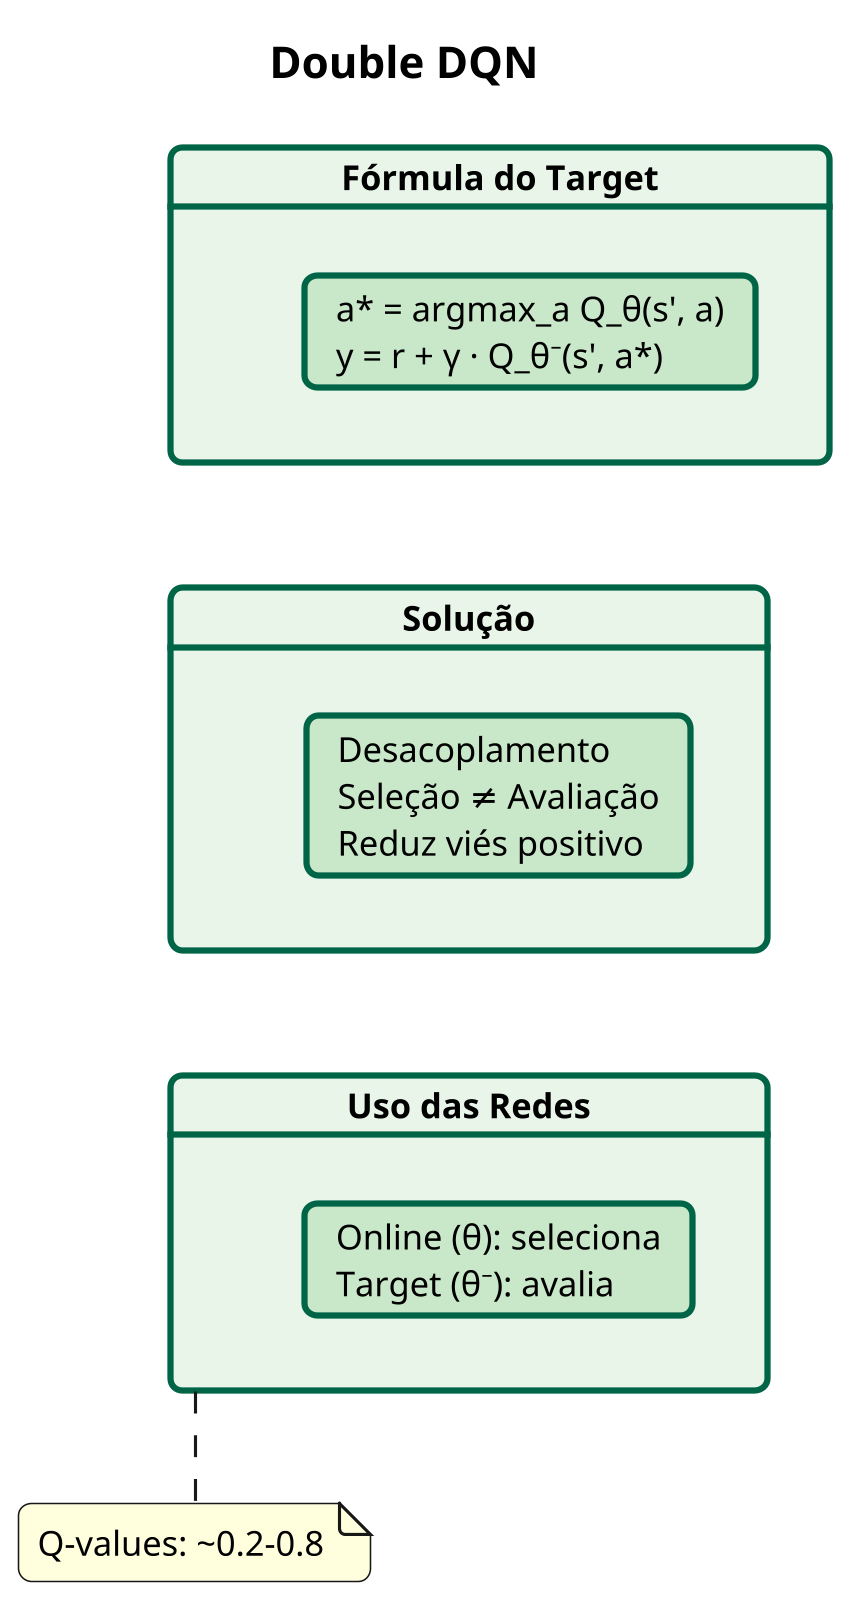
\includegraphics[width=0.95\textwidth,height=0.58\textheight,keepaspectratio]{double_dqn.png}
      \end{tcolorbox}
    \end{column}
  \end{columns}
  \vspace{2mm}
  \centering
  {\scriptsize \sutil{Double DQN desacopla seleção (online) de avaliação (target), reduzindo superestimação.}}
\end{frame}

% ======================================================
\section{Metodologia}
% ======================================================

\begin{frame}{Fluxo de um Episódio e Espaço de Ações}
  \vspace{-2mm}
  \begin{columns}[T]
    \begin{column}{0.42\textwidth}
      \centering
      % Diagrama: dqn_episode_flow.png
      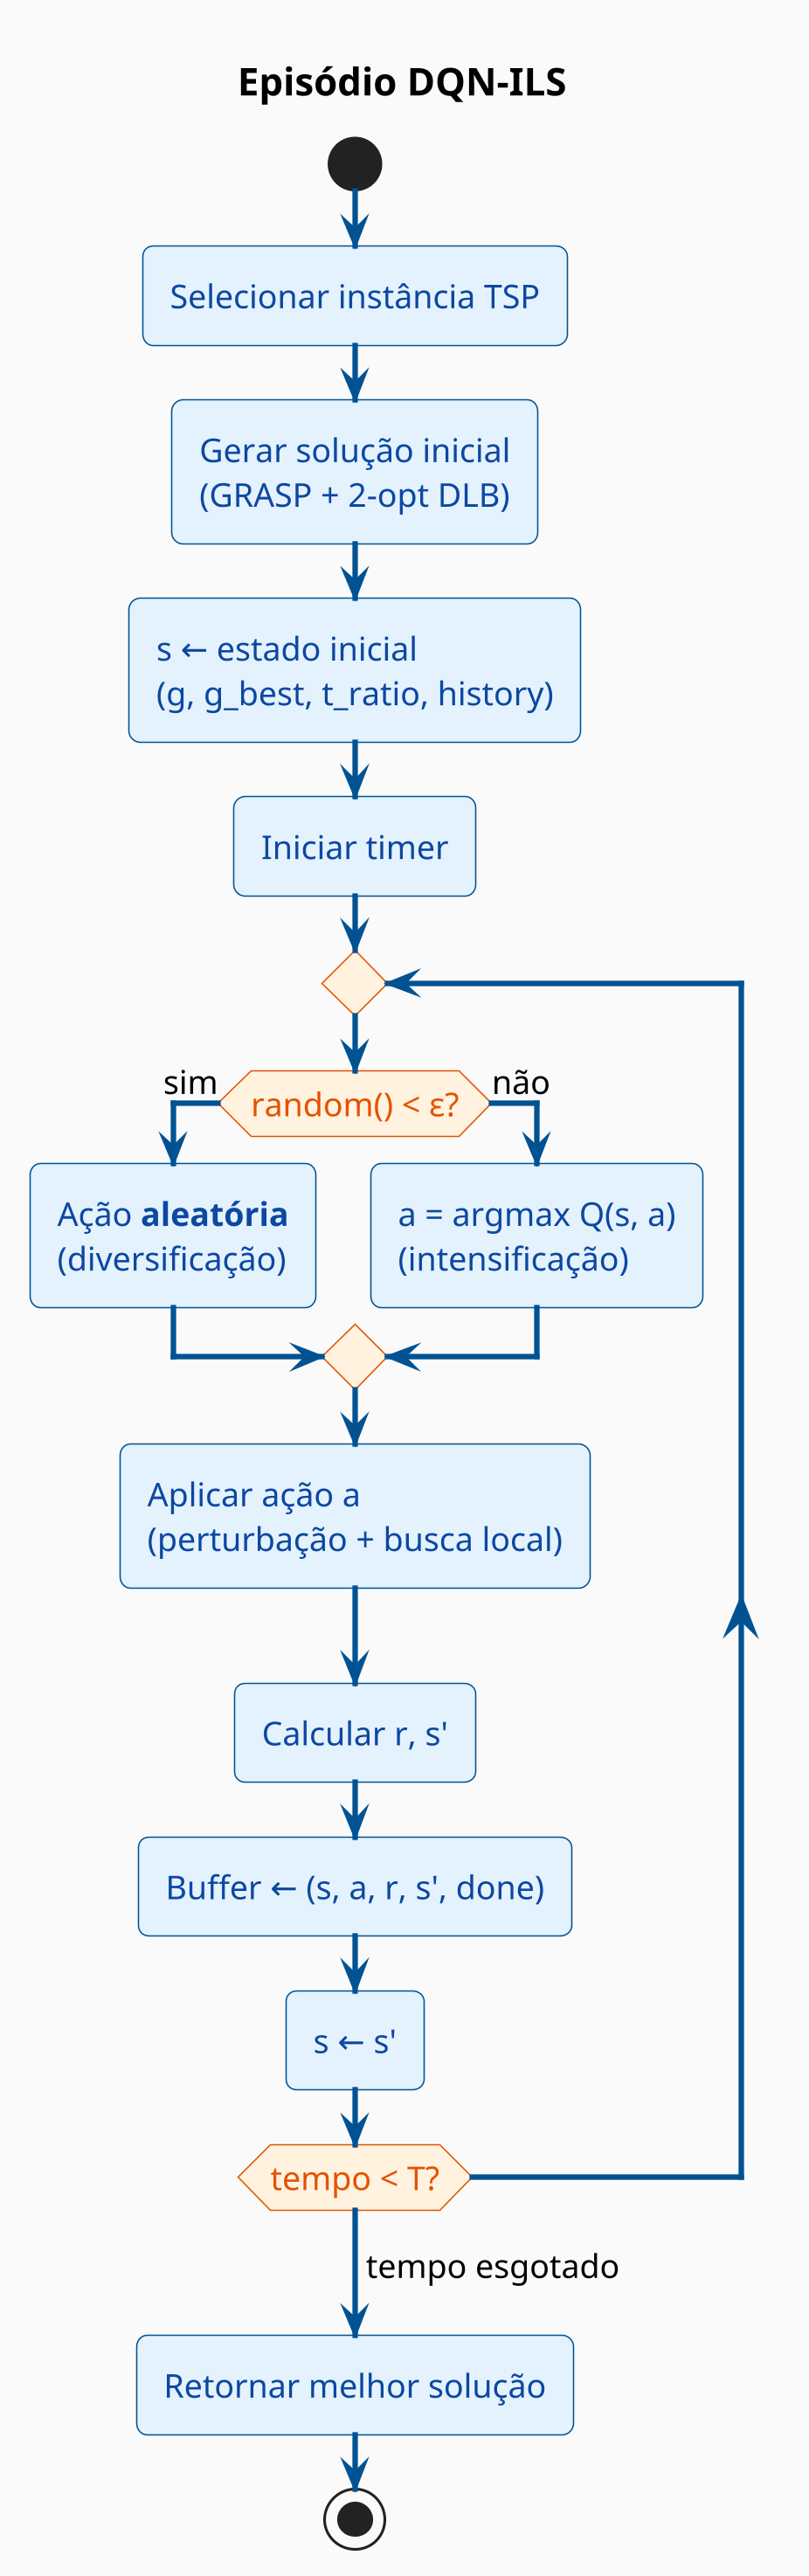
\includegraphics[width=\textwidth,height=0.85\textheight,keepaspectratio]{dqn_episode_flow.png}
    \end{column}
    \begin{column}{0.58\textwidth}
      \centering
      % Diagrama: dqn_action_space.png
      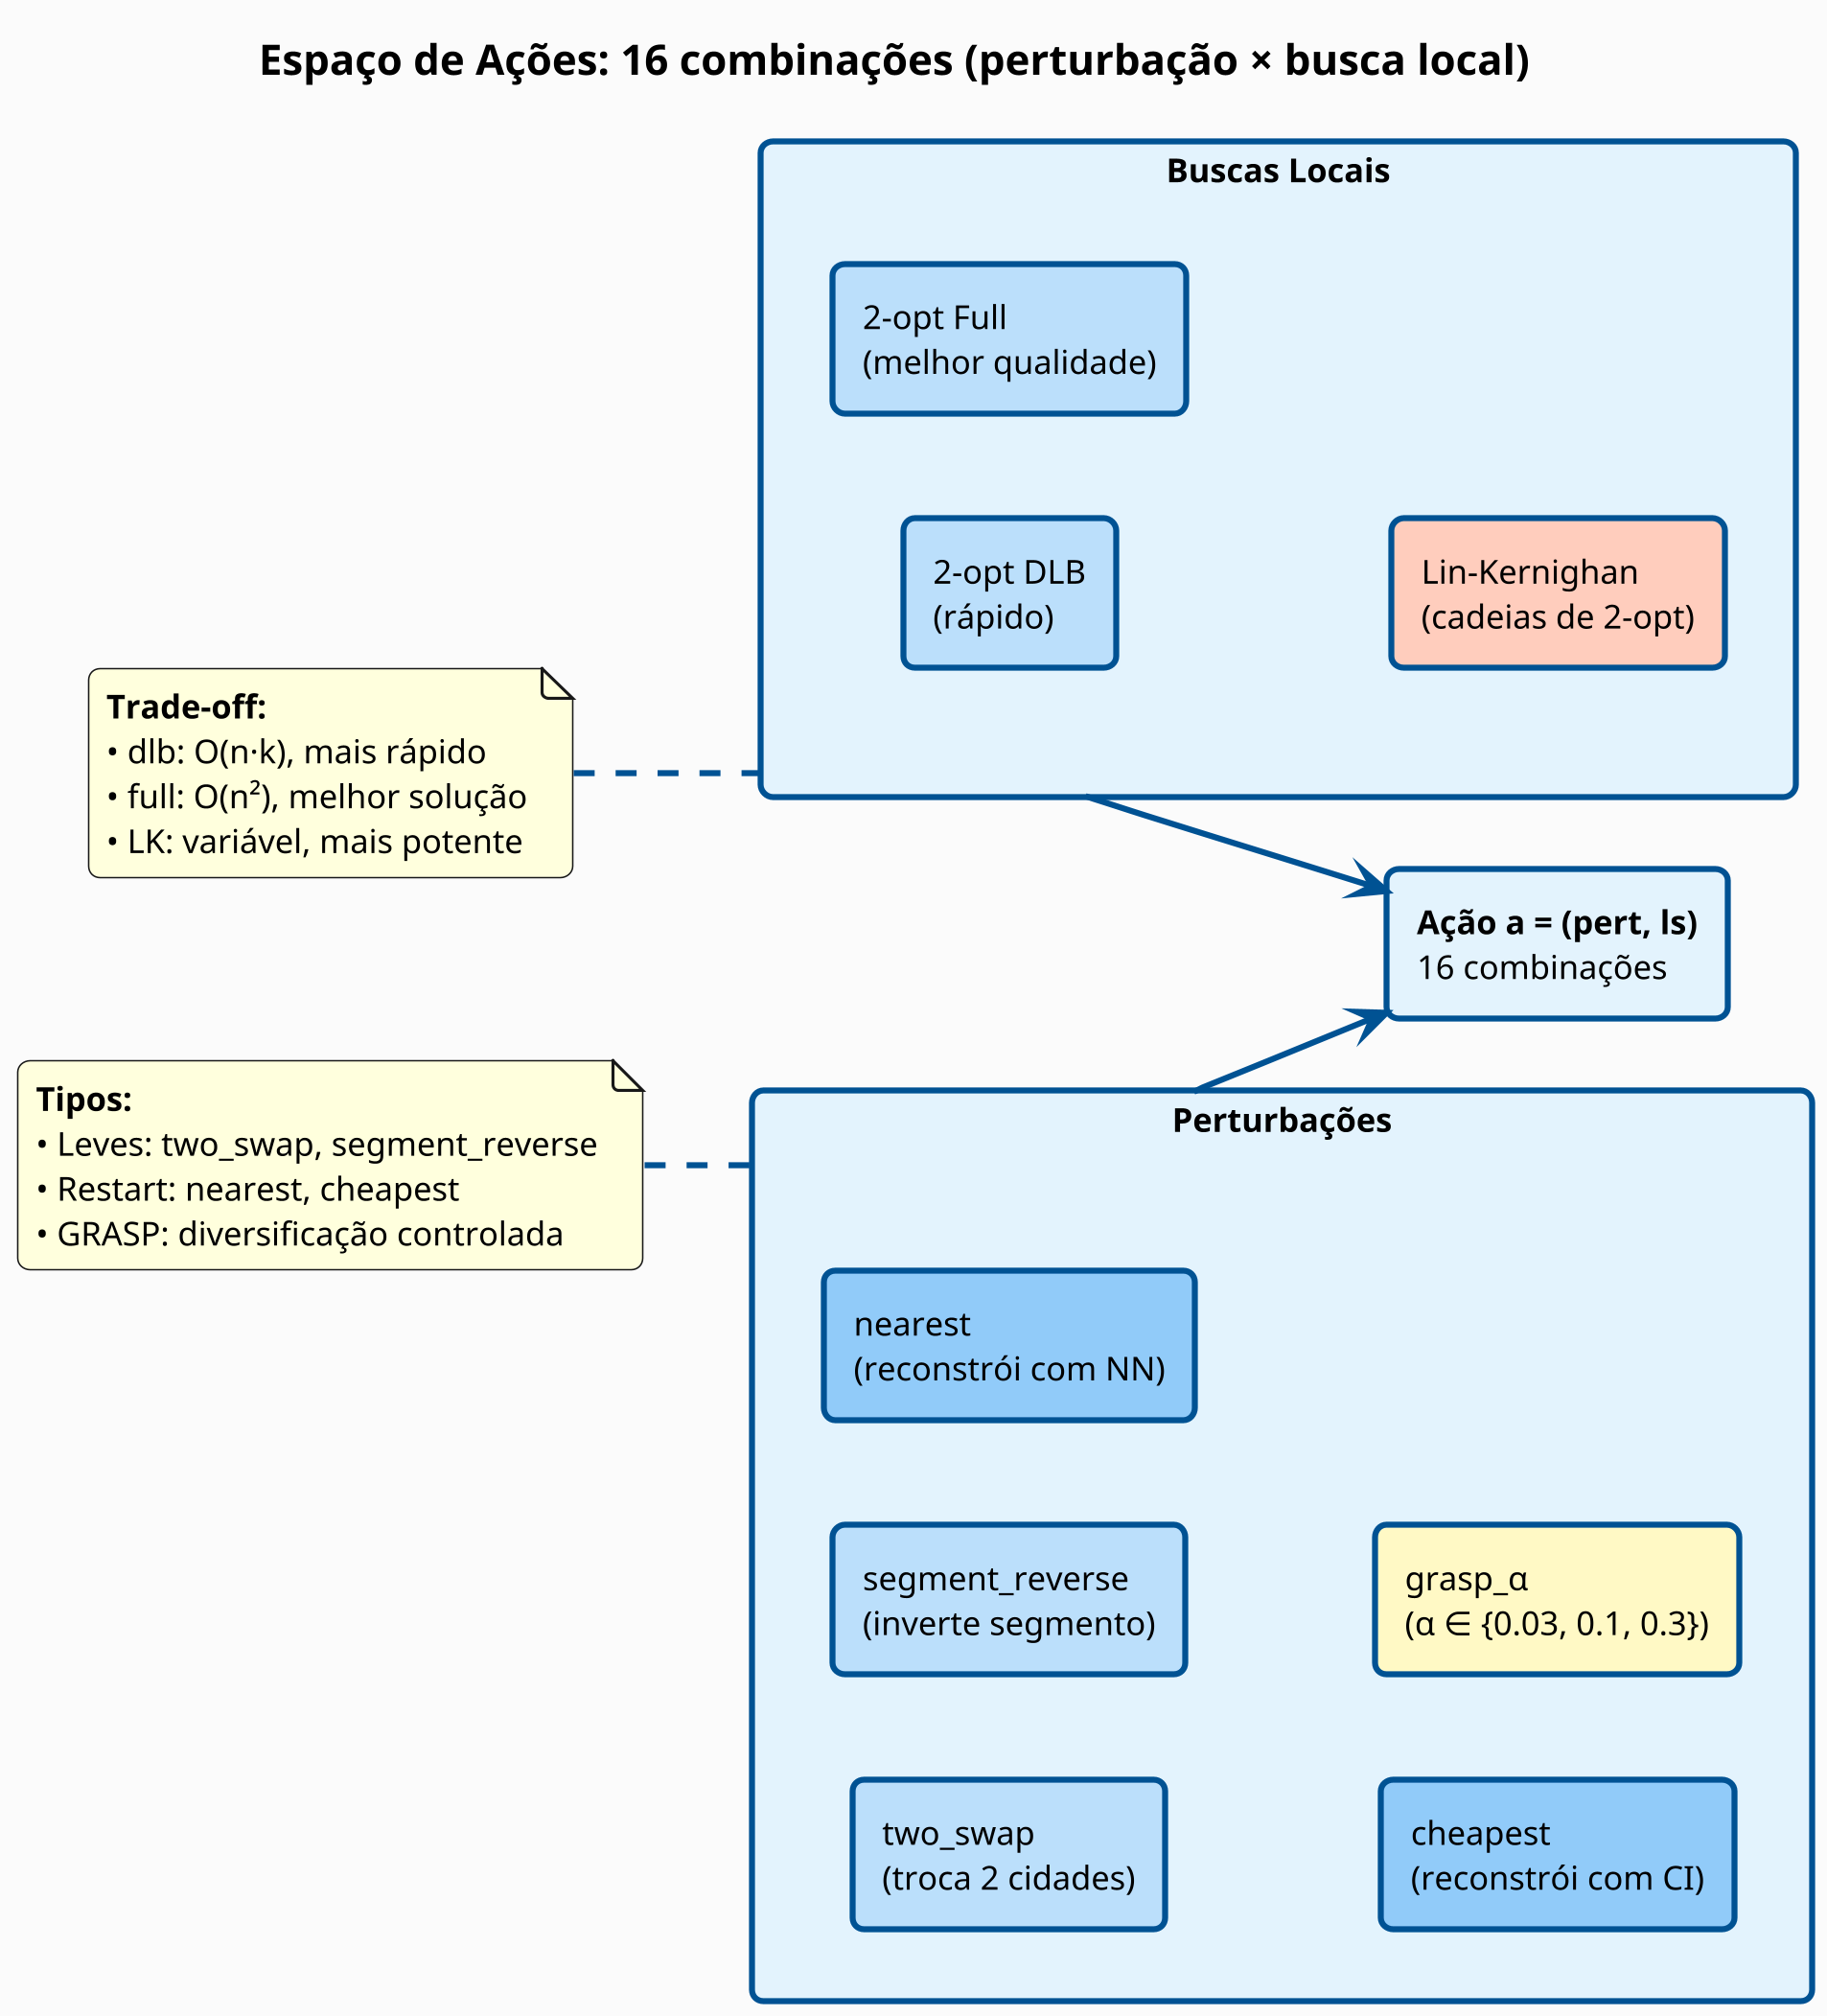
\includegraphics[width=\textwidth,height=0.85\textheight,keepaspectratio]{dqn_action_space.png}
    \end{column}
  \end{columns}
\end{frame}

\begin{frame}{Loop de Treinamento}
  \vspace{-3mm}
  \centering
  % Diagrama: dqn_training_loop.png
  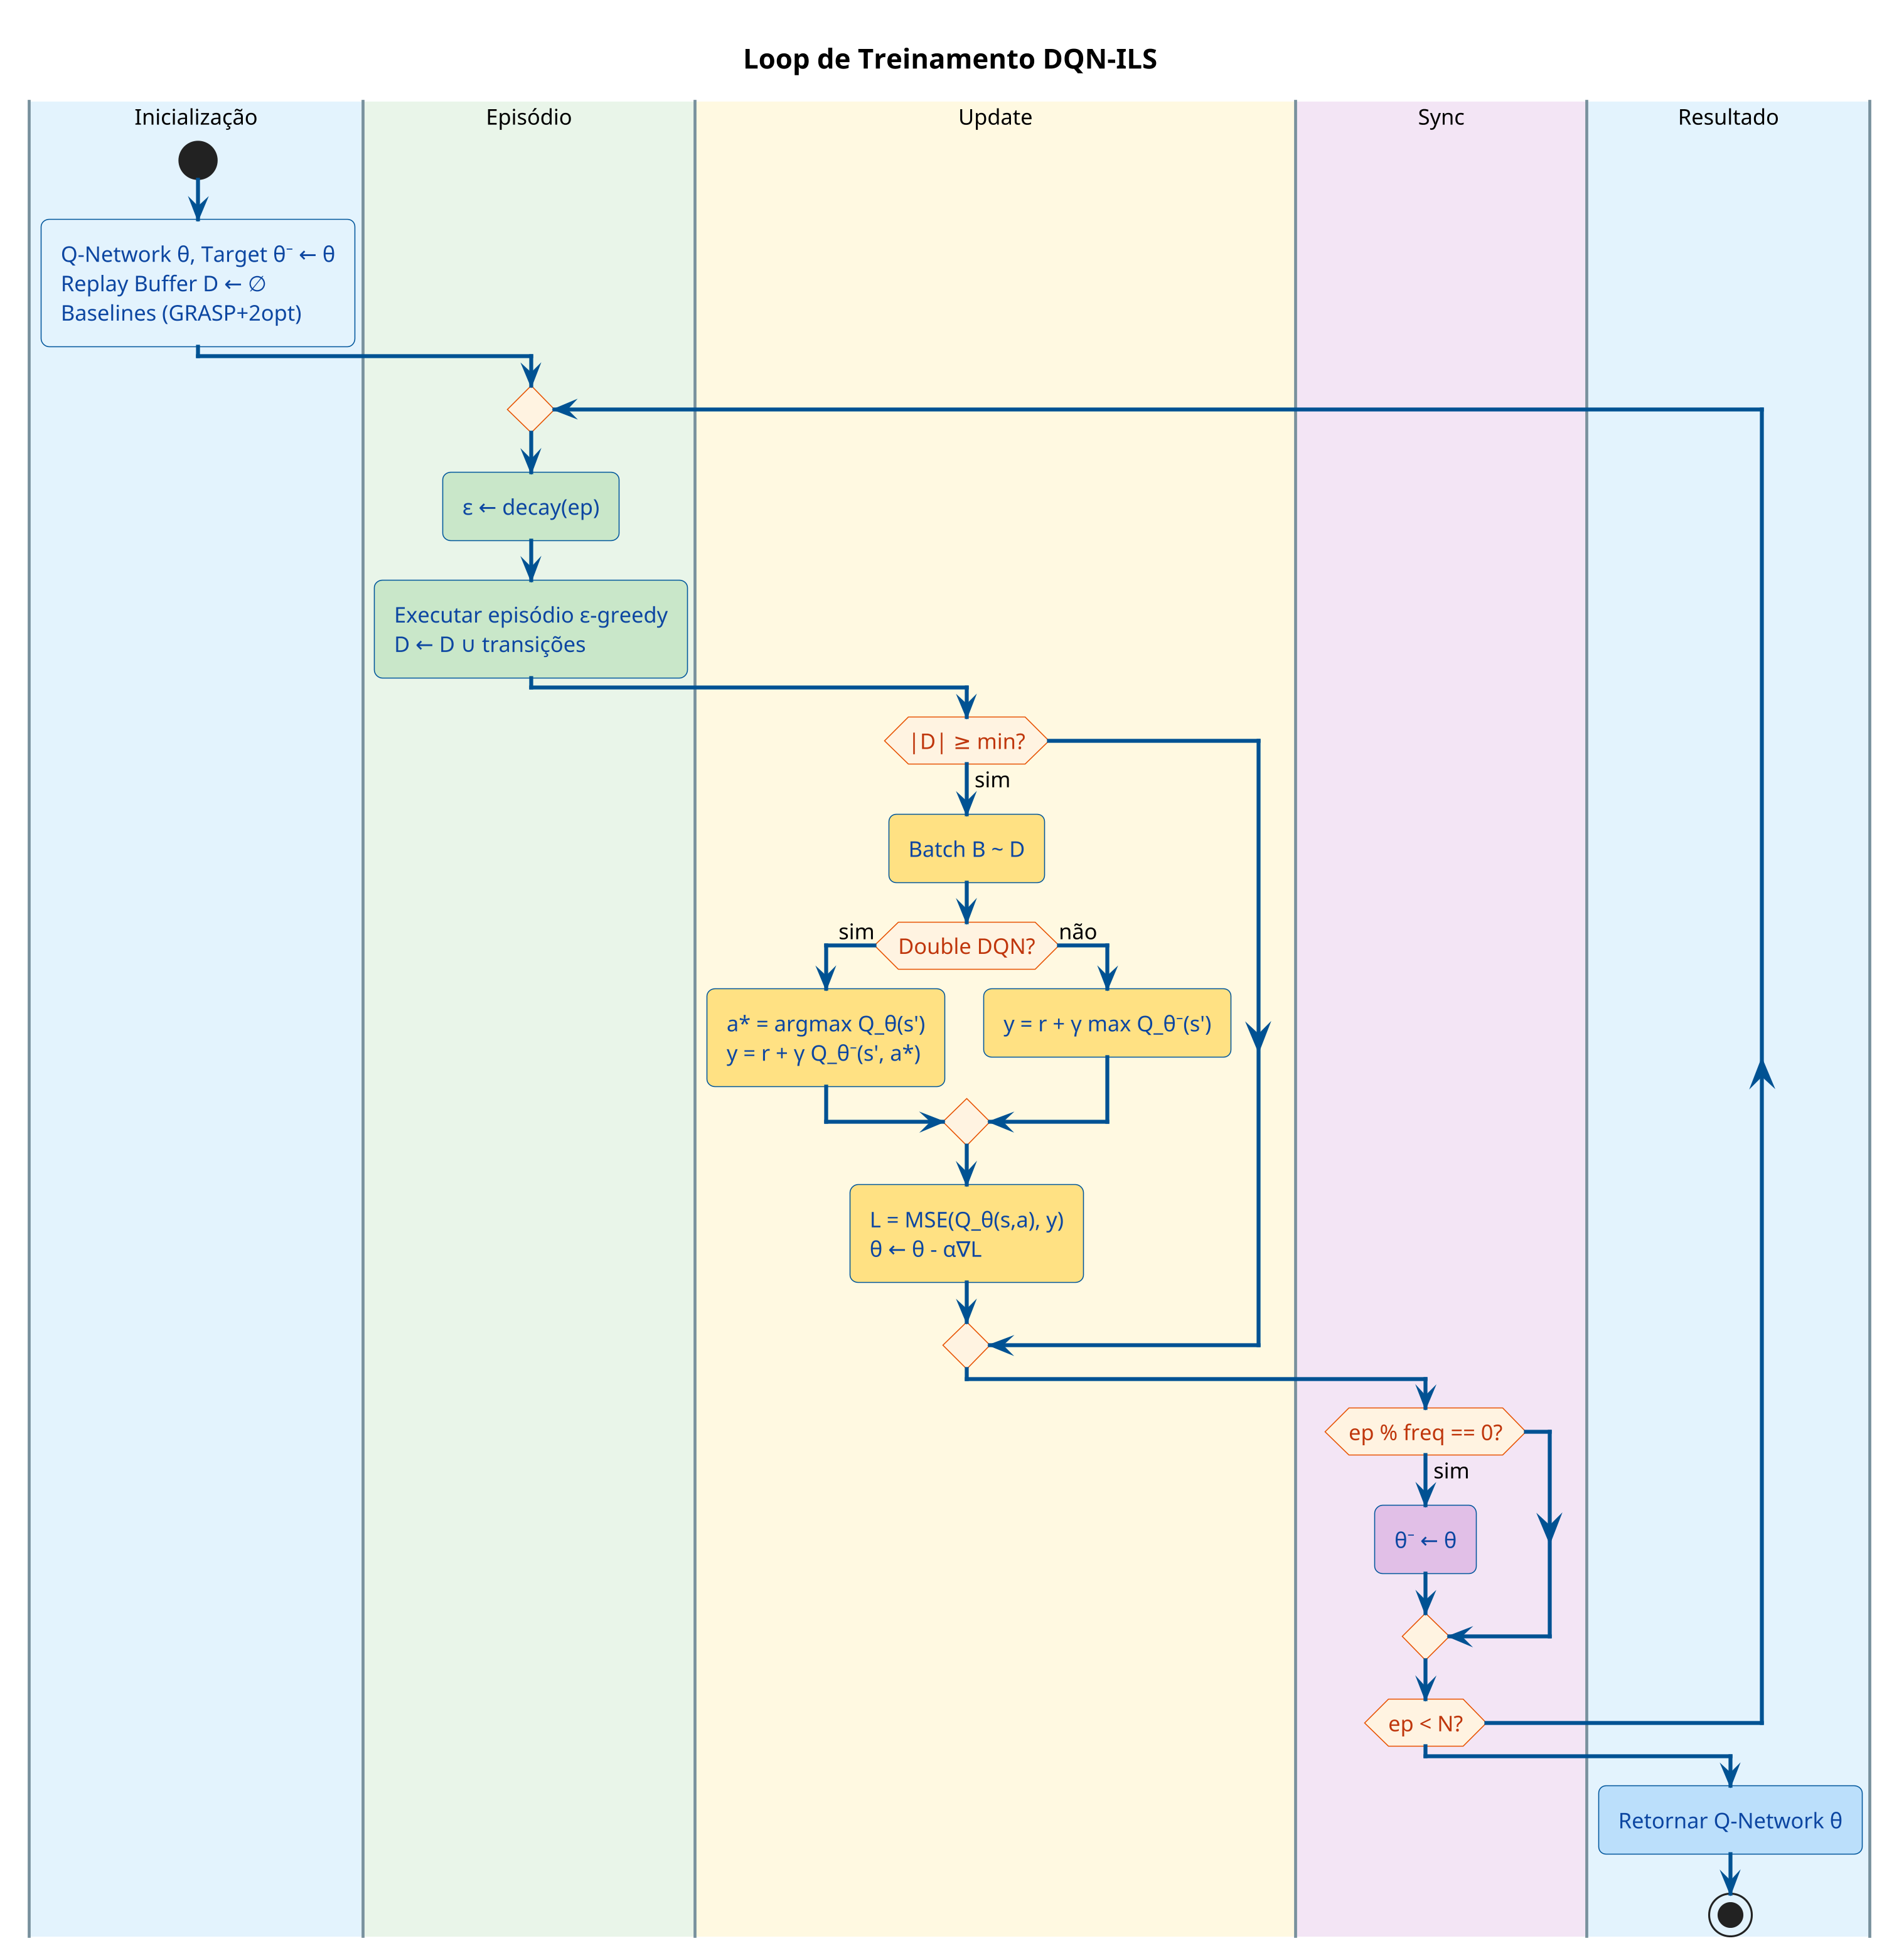
\includegraphics[width=0.8\textwidth,height=0.92\textheight,keepaspectratio]{dqn_training_loop.png}
\end{frame}

\begin{frame}{Sincronização da Target Network}
  \footnotesize
  \begin{columns}[T]
    \begin{column}{0.55\textwidth}
      \textbf{Duas redes no DQN:}
      \begin{itemize}
        \item \textbf{Online ($\theta$)}: atualizada a cada batch
        \item \textbf{Target ($\theta^-$)}: calcula targets $y$, atualizada \emph{periodicamente}
      \end{itemize}

      \vspace{2mm}
      \textbf{Hard update} (DQN clássico): \texttt{ep\%freq=0}
      \vspace{-2mm}
      \[
        \theta^- \leftarrow \theta \quad \text{\scriptsize (cópia total, freq=16 ep)}
      \]

      \vspace{1mm}
      \textbf{Soft update} (Polyak averaging, DDPG):
      \vspace{-2mm}
      \[
        \theta^- \leftarrow \tau \theta + (1-\tau) \theta^- \quad \text{\scriptsize ($\tau \approx 0.005$)}
      \]
      {\scriptsize Atualização gradual a cada passo. \\ Mais estável, sem tuning de período.}
    \end{column}
    \begin{column}{0.45\textwidth}
      \begin{alertbox}{Por que não atualizar sempre?}
        \scriptsize
        Se a target mudasse junto com a online, os targets $y$ seriam \textbf{alvos móveis}.

        \vspace{1mm}
        $\Rightarrow$ Instabilidade no treinamento

        \vspace{1mm}
        A separação temporal dá à rede online um \textbf{alvo fixo}, estabilizando o aprendizado.
      \end{alertbox}
      \vspace{2mm}
      {\scriptsize \sutil{Nossa implementação: hard update (padrão DQN).}}
    \end{column}
  \end{columns}
\end{frame}

\begin{frame}{Hiperparâmetros}
  \footnotesize
  \centering
  \renewcommand{\arraystretch}{1.2}
  \begin{tabular}{lcc}
    \toprule
    \textbf{Parâmetro} & \textbf{Valor} & \textbf{Descrição} \\
    \midrule
    $\gamma$ & 0.99 & Discount factor \\
    $\alpha$ (lr) & 0.0003 & Taxa de aprendizado \\
    hidden\_dim & 64 & Neurônios por camada \\
    batch\_size & 64 & Tamanho do batch \\
    buffer\_size & 50000 & Capacidade do replay buffer \\
    target\_update & 16 & Episódios entre updates \\
    $\epsilon_{\text{start}}$ & 1.0 & Diversificação inicial \\
    $\epsilon_{\text{end}}$ & 0.05 & Diversificação final \\
    \bottomrule
  \end{tabular}
  \vspace{3mm}

  \begin{calloutbox}
    {\scriptsize
    \textbf{$\epsilon$-decay logarítmico:} $\epsilon(t) = \epsilon_{\text{start}} \cdot \left(\frac{\epsilon_{\text{end}}}{\epsilon_{\text{start}}}\right)^{t/T}$
    }
  \end{calloutbox}
\end{frame}

% ======================================================
\section{Experimentos}
% ======================================================

\begin{frame}{Procedimento Experimental}
  \footnotesize
  \begin{columns}[T]
    \begin{column}{0.5\textwidth}
      \textbf{Instâncias:}
      \begin{itemize}
        \item Tipos: EUC\_2D, ATT, GEO
        \item Tamanhos: 10 a 100 vértices
        \item $\sim$11110 por tipo
        \item Split: 80\% treino, 10\% val, 10\% teste
      \end{itemize}
    \end{column}
    \begin{column}{0.5\textwidth}
      \textbf{Métricas:}
      \begin{itemize}
        \item Gap percentual ao ótimo
        \item Gap percentual ao baseline
        \item Q-values (monitoramento)
        \item Distribuição de ações
      \end{itemize}
      \vspace{2mm}
      \textbf{Ambiente:}
      \begin{itemize}
        \item Python + PyTorch
        \item Treinamento paralelo
      \end{itemize}
    \end{column}
  \end{columns}
\end{frame}

\begin{frame}{Resultado Principal}
  \footnotesize
  \vspace{-2mm}
  \begin{alertbox}
    {\footnotesize
    \textbf{Conclusão central:} O baseline GRASP+2opt é \destaque{consistentemente superior} ao DQN-ILS.
    }
  \end{alertbox}
  \vspace{2mm}

  \centering
  \renewcommand{\arraystretch}{1.3}
  \begin{tabular}{lccc}
    \toprule
    \textbf{Métrica} & \textbf{GRASP+2opt} & \textbf{DQN} & \textbf{Double DQN} \\
    \midrule
    Gap médio vs ótimo & \destaque{0.10\%} & 6.63\% & 3.99\% \\
    \% encontrando ótimo & \destaque{88.7\%} & 6.6\% & 15.8\% \\
    Vitórias head-to-head & \destaque{92.7\%} & 0.7\% & 0.8\% \\
    \bottomrule
  \end{tabular}

  \vspace{3mm}
  {\scriptsize \sutil{Dados: 600 instâncias de teste, EUC\_2D, n=20-70, 300 episódios de treino.}}

  \vspace{2mm}
  \begin{calloutbox}
    {\scriptsize
    \textbf{Interpretação:} O baseline multi-start é extremamente eficiente para TSP de pequeno/médio porte.
    O DQN-ILS não conseguiu aprender uma política superior.
    }
  \end{calloutbox}
\end{frame}

\begin{frame}{Resultados por Tamanho de Instância}
  \footnotesize
  \centering
  \renewcommand{\arraystretch}{1.2}
  \begin{tabular}{c|cc|cc|cc}
    \toprule
    & \multicolumn{2}{c|}{\textbf{GRASP+2opt}} & \multicolumn{2}{c|}{\textbf{DQN}} & \multicolumn{2}{c}{\textbf{Double DQN}} \\
    \textbf{n} & Gap & \% ópt & Gap & \% ópt & Gap & \% ópt \\
    \midrule
    20  & \destaque{0.19\%} & 93\% & 4.11\% & 21\% & 3.52\% & 33\% \\
    30  & \destaque{0.19\%} & 86\% & 6.51\% & 6\%  & 6.53\% & 4\%  \\
    40  & \destaque{0.04\%} & 97\% & 3.96\% & 5\%  & 4.18\% & 5\%  \\
    50  & \destaque{0.01\%} & 98\% & 9.36\% & 1\%  & 1.19\% & 35\% \\
    70  & \destaque{0.06\%} & 70\% & 9.20\% & 0\%  & 4.55\% & 2\%  \\
    100 & \destaque{0.30\%} & 19\% & 8.11\% & 0\%  & 6.31\% & 0\%  \\
    \bottomrule
  \end{tabular}

  \vspace{3mm}
  \begin{columns}[T]
    \begin{column}{0.5\textwidth}
      \begin{calloutbox}
        {\scriptsize
        \textbf{Baseline:} \\
        Quase ótimo para n$\leq$50 \\
        (86--98\% de taxa de sucesso)
        }
      \end{calloutbox}
    \end{column}
    \begin{column}{0.5\textwidth}
      \begin{alertbox}
        {\scriptsize
        \textbf{DQN Standard:} \\
        Gap cresce muito em n$\geq$50 \\
        (superestimação de Q-values)
        }
      \end{alertbox}
    \end{column}
  \end{columns}
\end{frame}

\begin{frame}{Standard DQN vs Double DQN: Q-values}
  \footnotesize
  \begin{columns}[T]
    \begin{column}{0.5\textwidth}
      \textbf{Evolução dos Q-values (n=70):}
      \vspace{2mm}

      \centering
      \renewcommand{\arraystretch}{1.2}
      \begin{tabular}{lcc}
        \toprule
        & \textbf{Standard} & \textbf{Double} \\
        \midrule
        Q\_mean início & 0.04 & 0.04 \\
        Q\_mean final & \textcolor{red}{1.48} & \destaque{0.56} \\
        Q\_max final & \textcolor{red}{2.31} & \destaque{0.82} \\
        \bottomrule
      \end{tabular}

      \vspace{3mm}
      {\scriptsize Standard DQN: Q-values explodem (superestimação).}
    \end{column}
    \begin{column}{0.5\textwidth}
      \textbf{Impacto na qualidade (n=50):}
      \vspace{2mm}

      \centering
      \renewcommand{\arraystretch}{1.2}
      \begin{tabular}{lcc}
        \toprule
        & \textbf{Standard} & \textbf{Double} \\
        \midrule
        Gap médio & 9.36\% & \destaque{1.19\%} \\
        \% ótimo & 1\% & \destaque{35\%} \\
        \bottomrule
      \end{tabular}

      \vspace{3mm}
      \begin{calloutbox}
        {\scriptsize
        \textbf{Double DQN $>$ Standard} \\
        Melhoria de 8pp no gap (n=50). \\
        \textbf{Mas perde para baseline.}
        }
      \end{calloutbox}
    \end{column}
  \end{columns}
\end{frame}

\begin{frame}{Por que o DQN-ILS falha?}
  \footnotesize
  \begin{columns}[T]
    \begin{column}{0.5\textwidth}
      \textbf{Hipótese 1: Problema ``fácil demais''}
      \begin{itemize}
        \item GRASP+2opt multi-start é quase ótimo para $n \leq 100$
        \item Espaço de busca pequeno o suficiente para heurísticas
        \item RL tem overhead sem vantagem compensatória
      \end{itemize}

      \vspace{3mm}
      \textbf{Hipótese 2: Estado pobre}
      \begin{itemize}
        \item Estado: $(g, g_{\text{best}}, t, \text{hist})$
        \item \textbf{Não inclui estrutura do tour}
        \item Rede não sabe \emph{quando} perturbar vs reiniciar
      \end{itemize}
    \end{column}
    \begin{column}{0.5\textwidth}
      \textbf{Hipótese 3: Ações mal balanceadas}
      \begin{itemize}
        \item 16 combinações com efeitos similares
        \item Difícil distinguir qual operador é melhor
        \item Política degenera (ex: 72\% mesma ação)
      \end{itemize}

      \vspace{3mm}
      \textbf{Hipótese 4: Reward inadequado}
      \begin{itemize}
        \item Delta reward: só premia ao melhorar recorde
        \item Maioria das ações $\rightarrow$ reward $\approx 0$
        \item Credit assignment difícil
      \end{itemize}
    \end{column}
  \end{columns}
\end{frame}

% ======================================================
\section{Conclusões}
% ======================================================

\begin{frame}{Discussão: O que Aprendemos}
  \footnotesize
  \begin{columns}[T]
    \begin{column}{0.5\textwidth}
      \textbf{Contribuições técnicas:}
      \begin{itemize}
        \item Framework DQN-ILS completo
        \item Comparação Standard vs Double DQN
        \item Análise de reward shaping
        \item Pipeline reprodutível
      \end{itemize}
      \vspace{2mm}
      \textbf{O que funcionou:}
      \begin{itemize}
        \item Double DQN reduz superestimação
        \item Generalização entre instâncias
        \item Baseline GRASP+2opt muito forte
      \end{itemize}
    \end{column}
    \begin{column}{0.5\textwidth}
      \textbf{O que não funcionou:}
      \begin{itemize}
        \item DQN-ILS não supera baseline
        \item Estado agregado insuficiente
        \item Overhead de inferência neural
        \item Escalabilidade limitada
      \end{itemize}
      \vspace{2mm}
      \begin{alertbox}
        {\scriptsize
        \textbf{Lição principal:} \\
        Para TSP $n \leq 100$, heurísticas multi-start são difíceis de superar com RL de alto nível.
        }
      \end{alertbox}
    \end{column}
  \end{columns}
\end{frame}

\begin{frame}{Conclusões}
  \footnotesize
  \begin{itemize}
    \item O \destaque{DQN-ILS} não é competitivo com GRASP+2opt para TSP de 20-100 nós.
    \item \destaque{Double DQN $>$ Standard DQN}: reduz superestimação, melhora estabilidade.
    \item O baseline GRASP+2opt é \destaque{surpreendentemente forte}: encontra ótimo em 88\% dos casos.
  \end{itemize}
  \vspace{3mm}
  \begin{calloutbox}
    {\footnotesize
    \textbf{Isso não significa que RL é inadequado para TSP:}
    \begin{itemize}
      \item A formulação MDP atual (estado agregado, ações de alto nível) não captura informação suficiente
      \item Para instâncias pequenas, heurísticas simples são difíceis de superar
      \item Abordagens \emph{end-to-end} (construir tour via RL) podem ser mais promissoras
    \end{itemize}
    }
  \end{calloutbox}
\end{frame}

\begin{frame}{Direções Futuras}
  \footnotesize
  \begin{columns}[T]
    \begin{column}{0.5\textwidth}
      \textbf{Se persistir com DQN-ILS:}
      \begin{itemize}
        \item Estado mais rico: features estruturais do tour (cruzamentos, distribuição de arestas)
        \item Espaço de ações simplificado: menos combinações, mais distintas
        \item Curriculum learning: instâncias progressivamente maiores
      \end{itemize}
    \end{column}
    \begin{column}{0.5\textwidth}
      \textbf{Alternativas mais promissoras:}
      \vspace{1mm}

      \centering
      \renewcommand{\arraystretch}{1.15}
      \begin{tabular}{ll}
        \toprule
        \textbf{Abordagem} & \textbf{Vantagem} \\
        \midrule
        PPO, A2C & Rewards esparsos \\
        GNN + RL & Tour como grafo \\
        Attention & Estado da arte \\
        \bottomrule
      \end{tabular}

      \vspace{3mm}
      {\scriptsize Pointer Networks (Vinyals et al., 2015) e Attention Model (Kool et al., 2019) constroem tours end-to-end.}
    \end{column}
  \end{columns}
\end{frame}

% ======================================================
\section*{Final}
% ======================================================

\begin{frame}{Referências}
  \evensmaller
  \begin{itemize}
    \item Mnih, V. et al. (2015).
          \textit{Human-level control through deep reinforcement learning}.
          Nature.
          \href{https://doi.org/10.1038/nature14236}{[doi]}
    \item van Hasselt, H., Guez, A., Silver, D. (2016).
          \textit{Deep Reinforcement Learning with Double Q-learning}.
          AAAI. \href{https://arxiv.org/abs/1509.06461}{arXiv:1509.06461}.
    \item Lillicrap, T. et al. (2016).
          \textit{Continuous control with deep RL} (DDPG, Polyak avg).
          ICLR. \href{https://arxiv.org/abs/1509.02971}{arXiv:1509.02971}.
    \item Vinyals, O. et al. (2015).
          \textit{Pointer Networks}.
          NeurIPS. \href{https://arxiv.org/abs/1506.03134}{arXiv:1506.03134}.
    \item Kool, W., van Hoof, H., Welling, M. (2019).
          \textit{Attention, Learn to Solve Routing Problems!}
          ICLR. \href{https://arxiv.org/abs/1803.08475}{arXiv:1803.08475}.
    \item Bengio, Y., Lodi, A., Prouvost, A. (2020).
          \textit{Machine Learning for Combinatorial Optimization}.
          \href{https://arxiv.org/abs/1811.06128}{arXiv:1811.06128}.
    \item Sutton, R. S., Barto, A. G. (2018).
          \textit{Reinforcement Learning: An Introduction}. MIT Press.
    \item OpenAI (2018).
          \textit{Spinning Up in Deep RL}.
          \href{https://spinningup.openai.com/}{spinningup.openai.com}.
  \end{itemize}
\end{frame}

\begin{frame}{Agradecimentos}
  \vfill
  \centering
  \adjustbox{height=0.3\textheight,keepaspectratio,interpolate}{
\includegraphics{panco.png}}
  \vspace{5mm}

  {\Large \destaque{Obrigado!}}
  \vspace{1cm}
\end{frame}

\end{document}
